\section{Screenshot Redmine}
\begin{figure}[H]
\centering
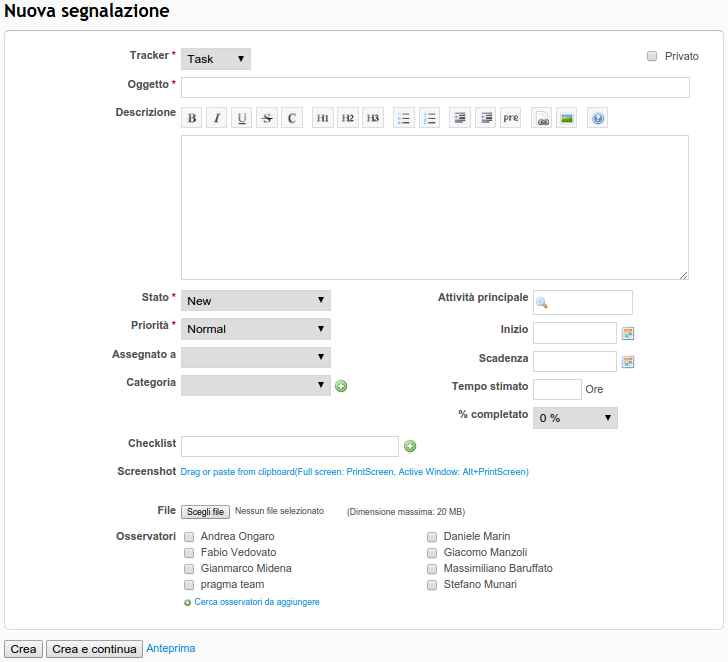
\includegraphics[width=14cm]{../immagini/nuovoTicket.png}
\caption{Form di creazione di un ticket}
\label{fig:assegnazioneTicket}
\end{figure}
%---------
\section{Screenshot \pragmadb}\label{screenPDB}
\begin{figure}[h]
\centering
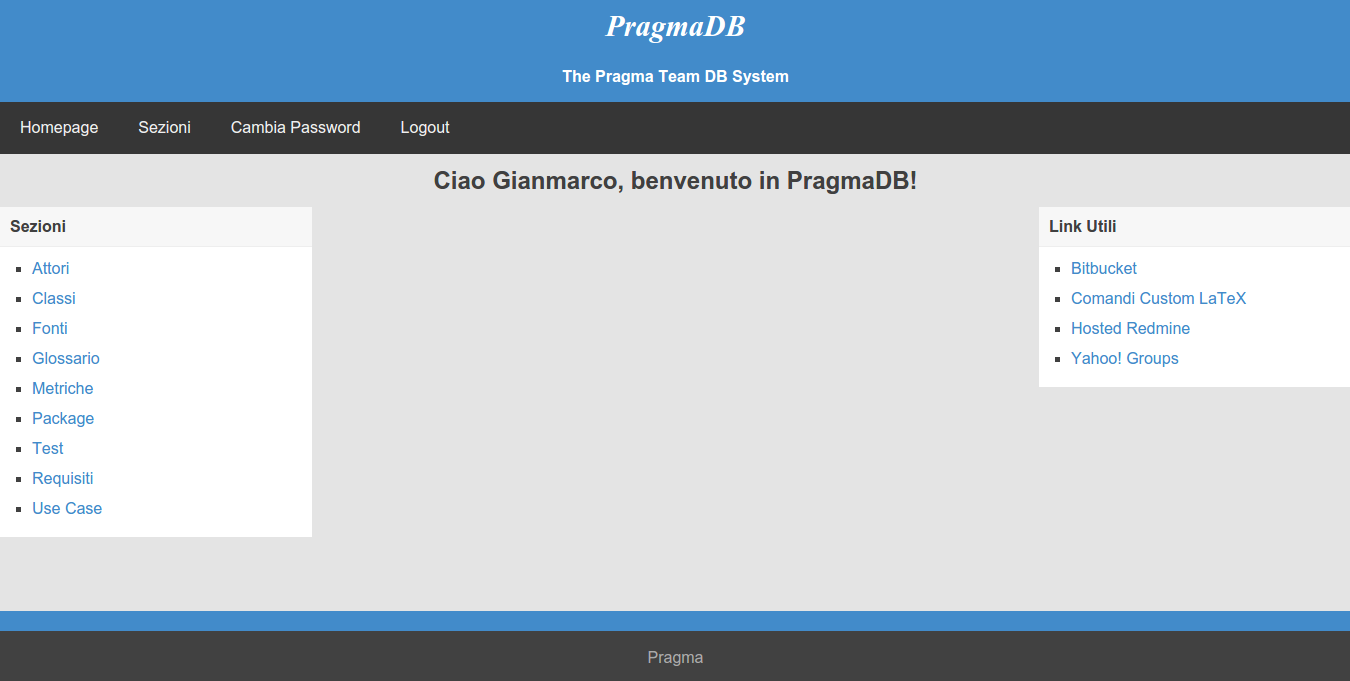
\includegraphics[width=\textwidth,keepaspectratio]{../immagini/home.png}
\caption{\pragmadb\ - pagina principale}\label{fig: PDBHome}
\end{figure}
%---------
\begin{figure}[h]
\centering
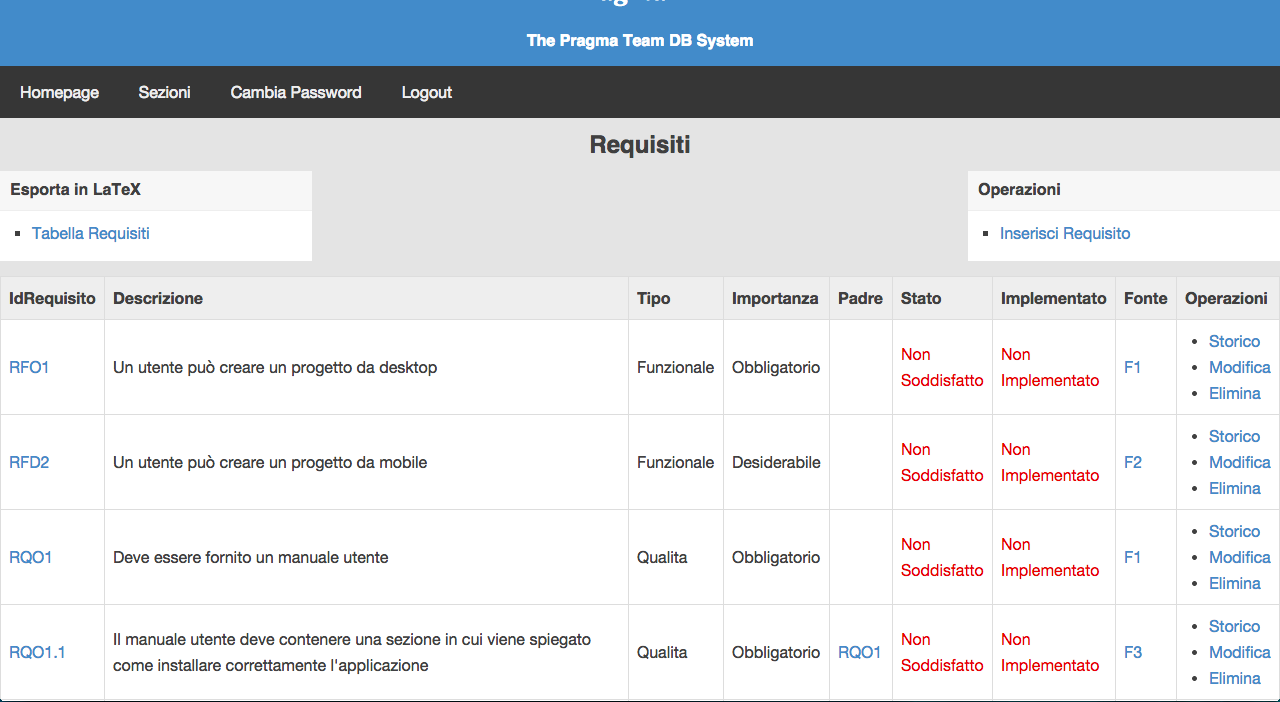
\includegraphics[width=\textwidth,keepaspectratio]{../immagini/requisiti.png}
\caption{\pragmadb\ - pagina dei requisiti}\label{fig: PDBRequisiti}
\end{figure}
%---------
\begin{figure}[h]
\centering
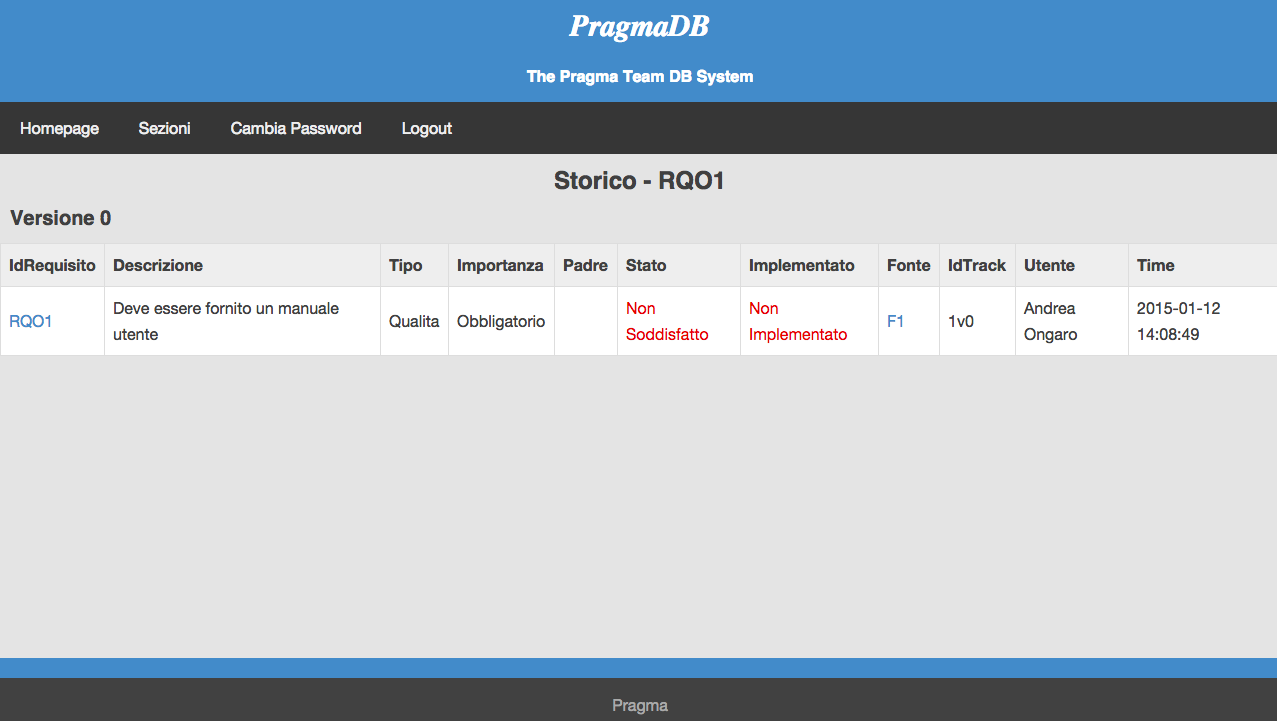
\includegraphics[width=\textwidth,keepaspectratio]{../immagini/history.png}
\caption{\pragmadb\ - pagina dello storico di uno specifico requisito}\label{fig: PDBHistory}
\end{figure}
%---------
\begin{figure}[h]
\centering
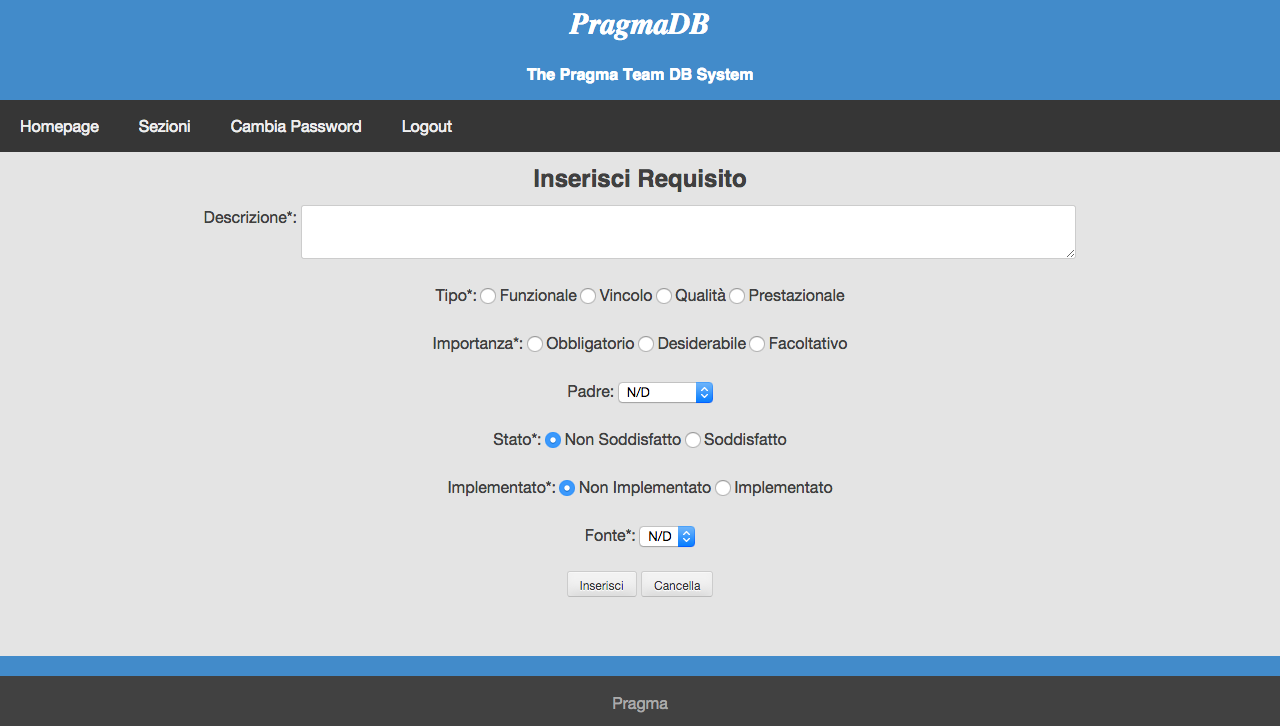
\includegraphics[width=\textwidth,keepaspectratio]{../immagini/insertReq.png}
\caption{\pragmadb\ - pagina di inserimento di un requisito}\label{fig: PDBInsert}
\end{figure}
%---------
\begin{figure}[h]
\centering
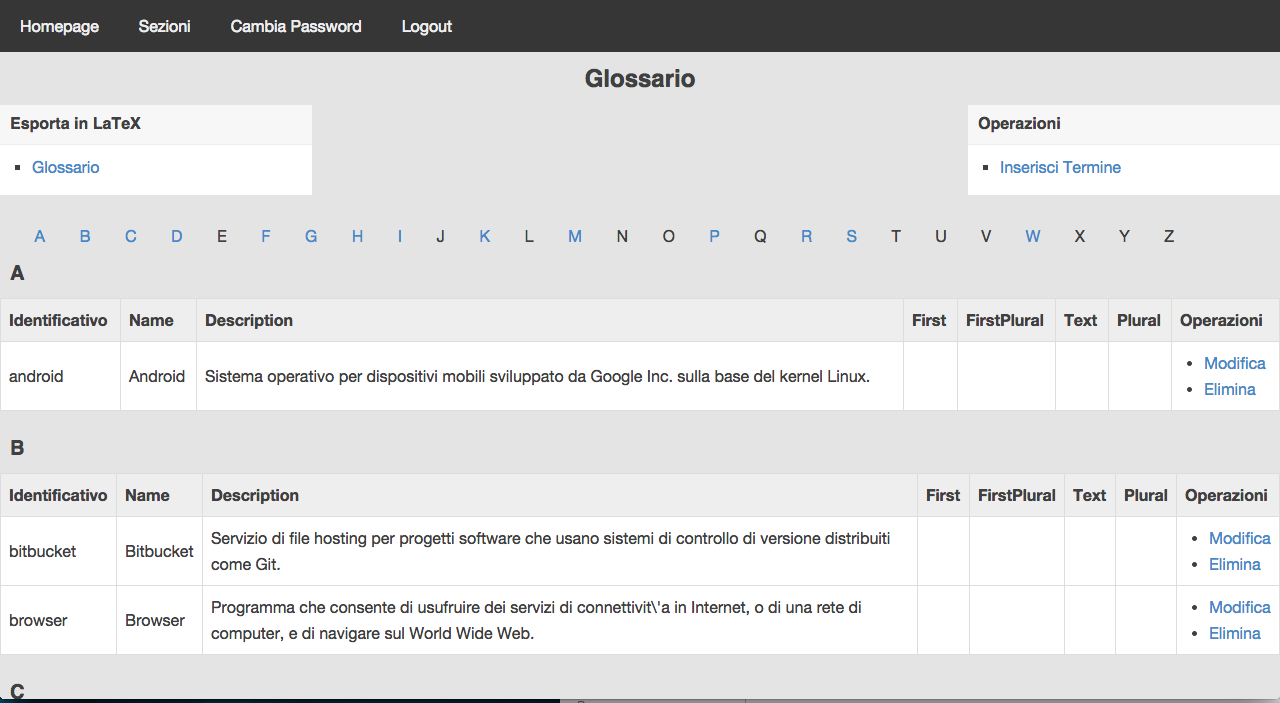
\includegraphics[width=\textwidth,keepaspectratio]{../immagini/glossario.png}
\caption{\pragmadb\ - pagina del \G}\label{fig: PDBGlossario}
\end{figure}
%---------
\begin{figure}[h]
\centering
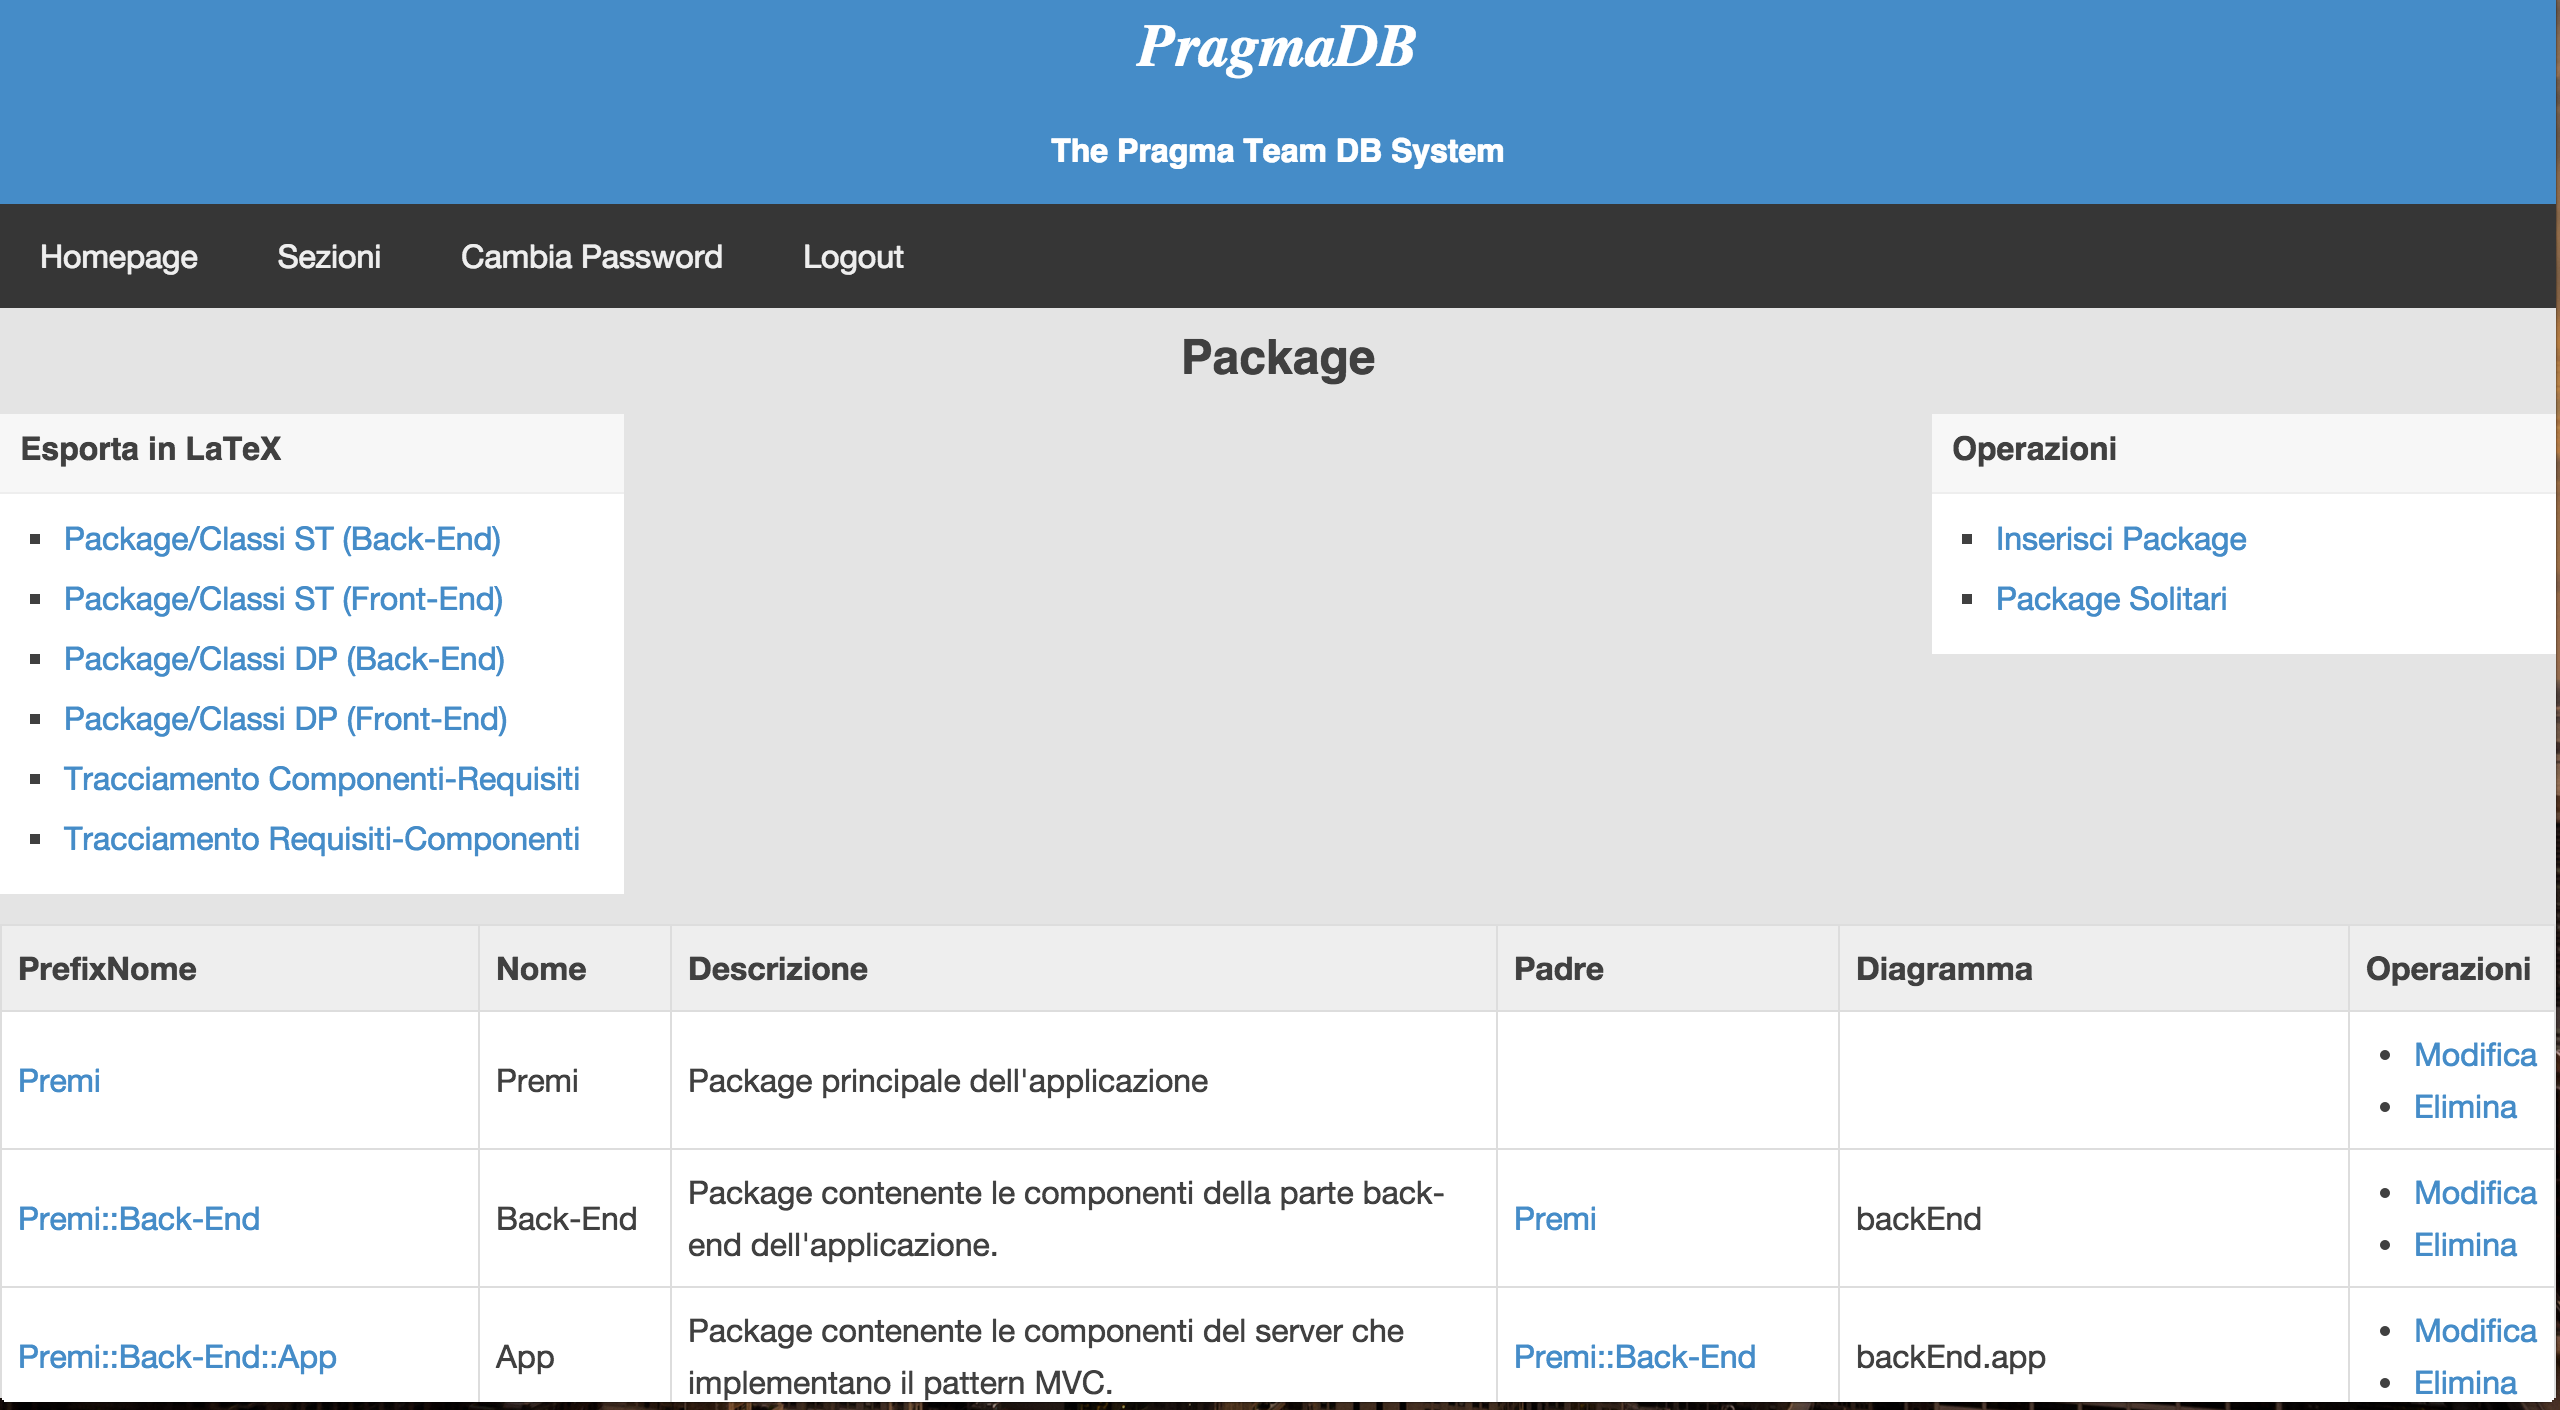
\includegraphics[width=\textwidth,keepaspectratio]{../immagini/pragmadbPackage.png}
\caption{\pragmadb\ - pagina dei package}\label{fig: PDBGlossario}
\end{figure}
%---------
\begin{figure}[h]
\centering
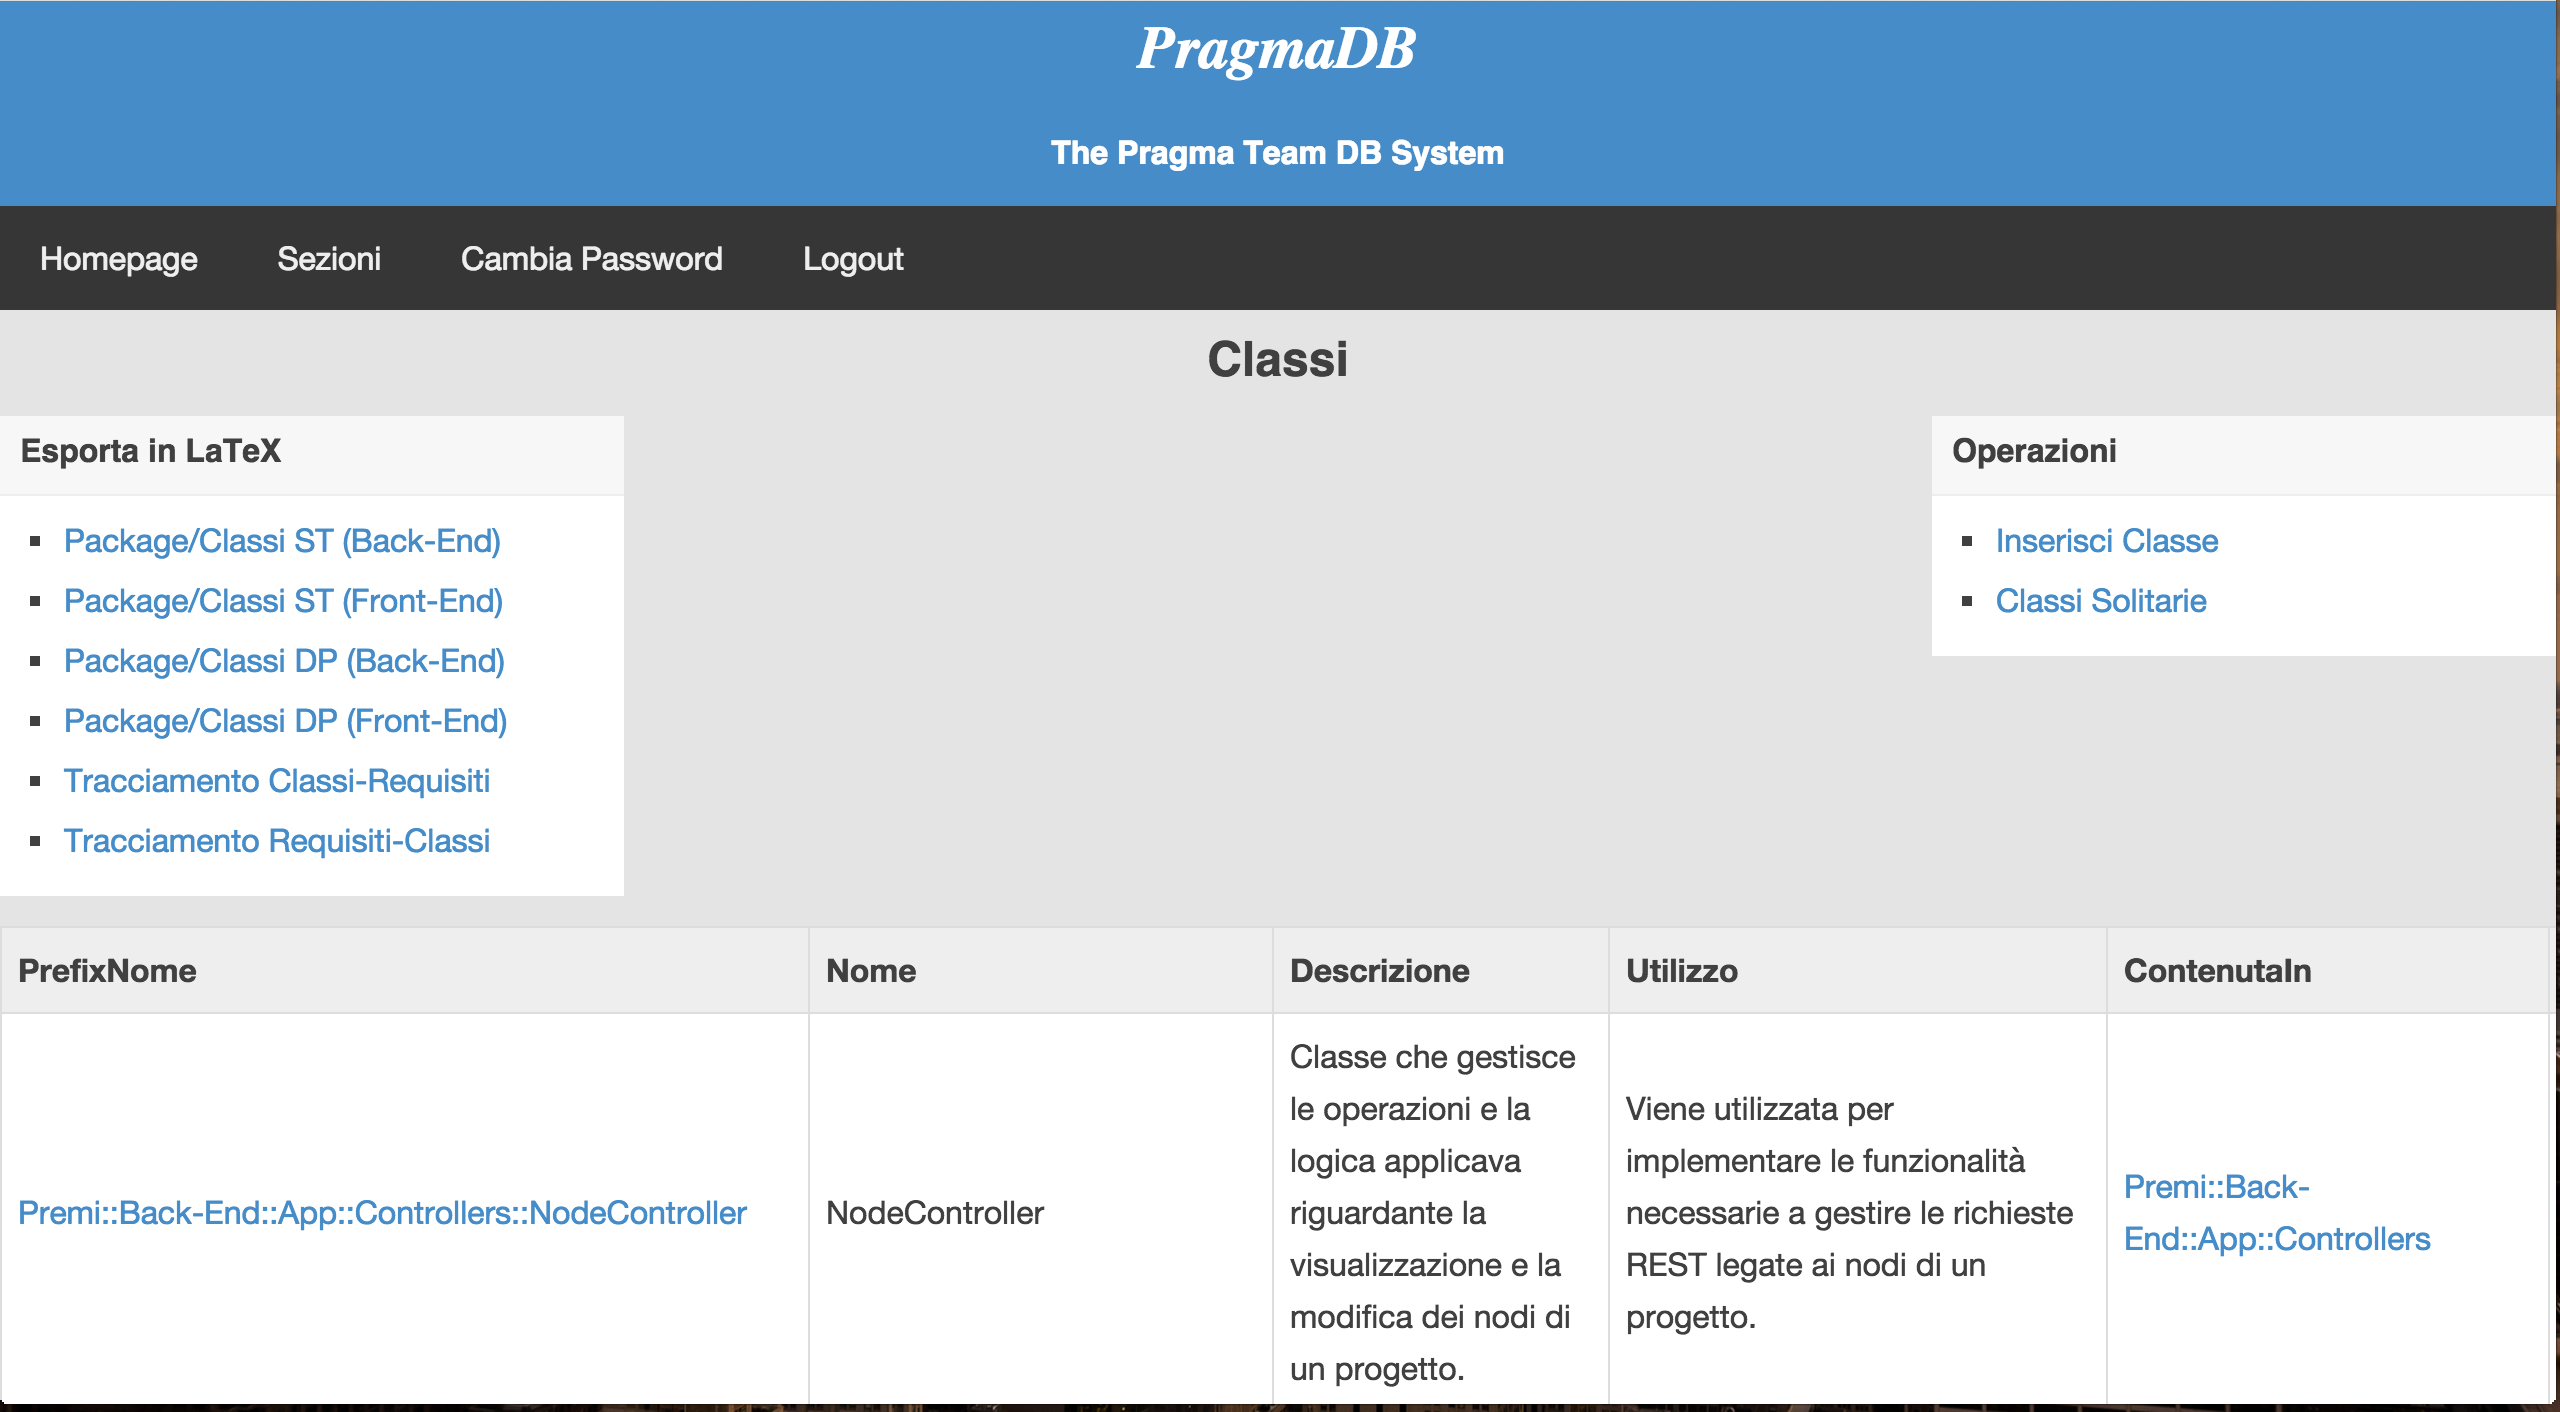
\includegraphics[width=\textwidth,keepaspectratio]{../immagini/pragmadbClassi.png}
\caption{\pragmadb\ - pagina delle classi}\label{fig: PDBGlossario}
\end{figure}
%---------
\begin{figure}[h]
\centering
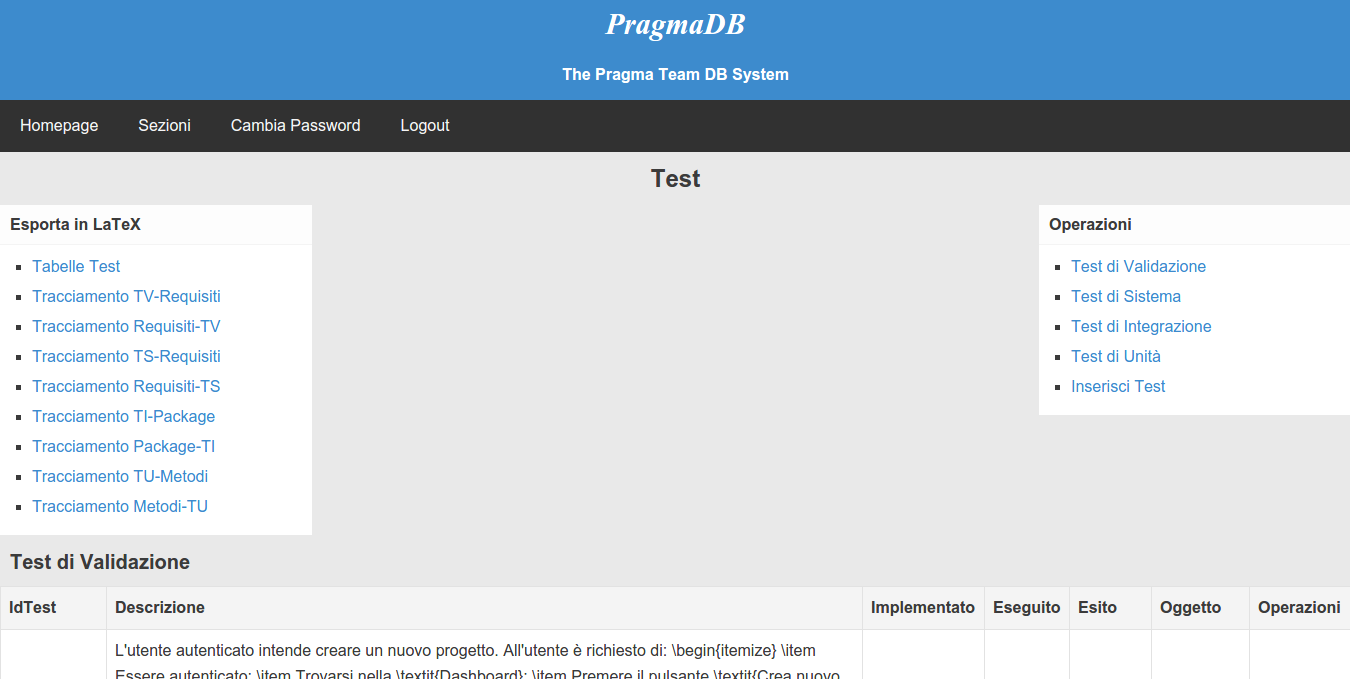
\includegraphics[width=\textwidth,keepaspectratio]{../immagini/pragmadbTest.png}
\caption{\pragmadb\ - pagina dei test}\label{fig: PDBTest}
\end{figure}
